\chapter{Blockchain}

\section*{Introduction}

In recent years, blockchain technology has emerged as a powerful tool for building trust, enhancing transparency, and decentralizing processes across various industries \cite{Nakamoto2008Bitcoin, Tapscott2016Blockchain}. In the context of Korpor, a platform aimed at facilitating real estate investments, blockchain plays a crucial role in ensuring the reliability and traceability of financial operations.

Traditional real estate investment systems often rely on centralized authorities and intermediaries, which may introduce delays, additional costs, or even fraudulent behavior. By integrating blockchain, Korpor addresses these limitations by recording key transactions such as investments, rent distributions, and project creation directly on a decentralized ledger \cite{Veuger2018RealEstateBlockchain}. This ensures that all stakeholders can verify actions in a transparent and immutable manner, without needing to trust a single party.

Moreover, smart contracts enable the automation of operations like rent distribution and investment validation, reducing human error and increasing efficiency \cite{Buterin2014Ethereum, Szabo1997SmartContracts}.

\section{Overview of Use Cases}

The blockchain integration within the \textbf{\textcolor{primary}{Korpor}} platform addresses several core functionalities that benefit from decentralization and transparency. The main use cases implemented include:

\begin{itemize}
    \item \textbf{Investment Recording}
    \begin{itemize}
        \item Immutable proof of ownership for the investor.
        \item Transparent public records of all investment flows.
        \item Verifiable data for audits or external reviews.
    \end{itemize}

    \item \textbf{Project Registration}
    \begin{itemize}
        \item Proof of project existence on-chain.
        \item Traceability of project updates and funding status.
        \item Protection against unauthorized modifications.
    \end{itemize}

    \item \textbf{Rent Distribution}
    \begin{itemize}
        \item Calculate and distribute rental income fairly to investors.
        \item Automate distribution without manual intervention.
        \item Log each rent payout on the blockchain for transparency.
    \end{itemize}

    \item \textbf{Transaction Verification}
    \begin{itemize}
        \item Trust in the platform.
        \item User empowerment to track their funds and participation.
        \item Regulatory compliance through transparent financial trails.
    \end{itemize}
\end{itemize}

\section{Objectives of Blockchain Integration}

The integration of blockchain technology into the \textbf{\textcolor{primary}{Korpor}} platform serves several key objectives aimed at enhancing the system's reliability, transparency, and automation capabilities:

\begin{itemize}
    \item \textbf{Security and trust in transactions}
    \begin{itemize}
        \item Ensures that each transaction is securely signed and verified.
        \item Builds trust among users by preventing unauthorized modifications \cite{Zheng2018BlockchainChallenges}.
        \item Enhances transparency through verifiable on-chain records.
    \end{itemize}

    \item \textbf{Decentralization and immutability}
    \begin{itemize}
        \item Eliminates single points of failure by distributing data across the blockchain.
        \item Guarantees that data, once written, cannot be altered \cite{Antonopoulos2018MasteringEthereum}.
        \item Promotes resilience and long-term reliability of the system.
    \end{itemize}

    \item \textbf{Automation through smart contracts}
    \begin{itemize}
        \item Enables automatic execution of business logic (e.g., rent distribution) \cite{Bartoletti2017EmpiricalAnalysis}.
        \item Reduces manual intervention and human error.
        \item Increases system efficiency through self-executing contracts.
    \end{itemize}
\end{itemize}

\section{Technical Architecture}

The blockchain component is designed to integrate seamlessly within the overall architecture of the \textbf{\textcolor{primary}{Korpor}} platform. This section outlines how the blockchain fits into the system and the technologies used for its implementation.

\begin{itemize}
    \item \textbf{How blockchain fits into the overall system architecture}
    \begin{itemize}
        \item The backend communicates with smart contracts deployed on the Ethereum blockchain.
        \item Transactions such as investments, project registrations, and rent distributions are processed and recorded on-chain.
        \item The blockchain acts as a complementary layer to ensure data integrity and traceability.
    \end{itemize}

    \item \textbf{On-chain vs off-chain components}
    \begin{itemize}
        \item \textit{On-chain:}
        \begin{itemize}
            \item Smart contracts handle investments, project registrations, and rent distributions.
            \item Data recorded on-chain is immutable and publicly verifiable.
        \end{itemize}
        \item \textit{Off-chain:}
        \begin{itemize}
            \item User data, authentication, and detailed analytics are managed by the backend and stored in a centralized database (MySQL).
            \item Interaction with the blockchain is facilitated through API endpoints and external services \cite{Xu2019ArchitectingBlockchainApplications}.
        \end{itemize}
    \end{itemize}

    \item \textbf{Technologies used}
   \begin{itemize}
    \item 
\includegraphics[width=0.05\textwidth]{images/icons/solidity.png} \textbf{Solidity:} A high-level programming language specifically designed for writing secure, efficient, and decentralized smart contracts on the Ethereum blockchain \cite{SolidityDocs}.
    
    \item 
\includegraphics[width=0.05\textwidth]{images/icons/etherscan.png} \textbf{Ethers.js:} A popular JavaScript library used to interact with the Ethereum blockchain, providing functionality to manage accounts, send transactions, and call smart contract functions \cite{EthersJSDocs}.
    
    \item 
\includegraphics[width=0.05\textwidth]{images/icons/sepolia.png} \textbf{Sepolia Testnet:} A test network for Ethereum that allows developers to deploy and test their smart contracts in a safe, controlled environment without spending real cryptocurrency.
    
    \item 
\includegraphics[width=0.05\textwidth]{images/icons/infura.png} \textbf{Infura:} A cloud-based platform that provides access to Ethereum nodes via JSON-RPC, eliminating the need to run a full Ethereum node \cite{InfuraWeb3}.
    
    \item 
\includegraphics[width=0.05\textwidth]{images/icons/metamask.png} \textbf{MetaMask:} A widely-used browser extension and mobile application that serves as a cryptocurrency wallet for interacting with decentralized applications \cite{MetaMaskDocs}.
   \end{itemize}
\end{itemize}

\subsection{Third-Party Payment Integration: Paymee}

In the Korpor platform, secure and reliable payment processing is fundamental to enabling users to invest in real estate projects with confidence. While blockchain handles transparency and decentralization for on-chain interactions, fiat payments from users need to be handled via trusted third-party providers. For this purpose, we chose \textbf{Paymee} as our main payment gateway.

% Placeholder for Paymee Framework diagram
\begin{figure}[htbp]
\centering
% PLACEHOLDER: Insert Paymee Framework diagram here

\includegraphics[width=0.8\textwidth]{images/paymee_framework.png}
\caption{Paymee Framework}
\label{fig:paymee-framework}
\end{figure}

\subsubsection{Role of Paymee in the Architecture}

Paymee acts as a bridge between the user's traditional banking system and our decentralized investment platform. When a user decides to invest in a project, the fiat transaction is processed securely via Paymee. Upon confirmation, the platform triggers an on-chain event that records the investment using a smart contract, ensuring both real-world and blockchain-level consistency.

\begin{itemize}
    \item Paymee provides a secure and verified method for processing payments via bank cards or wallets.
    \item It offers real-time transaction status updates, which are essential for synchronizing with blockchain confirmations.
    \item The integration ensures that only successful payments are recorded on-chain, reducing fraud and improving traceability \cite{Bamakan2020BlockchainPayment}.
\end{itemize}

\subsubsection{Justifying the Choice of Paymee}

Several third-party payment providers are available in Tunisia, including  \textbf{Flouci} 
\includegraphics[width=0.05\textwidth]{images/icons/flouci_icon.png} and  \textbf{Konnect} 
\includegraphics[width=0.05\textwidth]{images/icons/konnect_icon.png} , however, \textbf{Paymee} was chosen due to its distinct advantages in several key areas:

\begin{itemize}
  \item \textbf{Regulatory Compliance:} Fully compliant with local regulations and has established partnerships with most major Tunisian banks.
  
  \item \textbf{Developer Experience:} Offers clear documentation, a stable sandbox environment, and responsive customer support.
  
  \item \textbf{Payment Mode:} Supports a wide range of payment methods, including both local and international options.
  
  \item \textbf{Pricing:} Offers simplified and transparent pricing with competitive rates.
  
  \item \textbf{User Experience:} Provides a minimalistic and intuitive user interface that reduces drop-off rates during transactions.
  
  \item \textbf{Flexibility:} Highly flexible and easily integrates into diverse use cases, adapting to the requirements of individual investors.
\end{itemize}
\newpage
% Placeholder for Payment Providers Comparison Table
\begin{table}[htbp]
\centering
\caption{Comparison of Payment Providers: Paymee vs Flouci vs Konnect}
\label{tab:payment_comparison}
\begin{tabular}{|p{4cm}|p{3.5cm}|p{3.5cm}|p{3.5cm}|}
\hline
\textbf{Feature} & \textbf{Paymee} & \textbf{Flouci} & \textbf{Konnect} \\ \hline
\textbf{Regulatory Compliance} & Fully compliant with local regulations & Limited compliance & Enterprise-focused, may have specific requirements \\ \hline
\textbf{Developer Experience} & Clear documentation, stable sandbox, responsive support & Less stable APIs, limited documentation & Lengthy onboarding, limited flexibility \\ \hline
\textbf{Payment Model} & Ideal for recurring, high-trust investments & Not suited for investment models & Enterprise-focused with fixed pricing \\ \hline
\textbf{Pricing} & Simplified and transparent & Unclear pricing structure & Complex pricing and fees \\ \hline
\textbf{User Experience} & Minimalistic UI, reliable webhooks, low drop-offs & Less reliable, mobile payment focus & Enterprise UI, longer process, limited customization \\ \hline
\textbf{Flexibility} & High flexibility in fee structures & Low flexibility & Low flexibility, rigid fee structures \\ \hline
\end{tabular}
\end{table}

Based on these factors, \textbf{Paymee} was selected as the most suitable payment provider for the Korpor platform, playing a pivotal role in bridging traditional finance with our blockchain-based investment infrastructure.

\section{Smart Contract Design}

\subsection{Smart Contracts Overview}

A smart contract is a self-executing contract with the terms of the agreement directly written into lines of code \cite{Szabo1997SmartContracts}. These contracts run on blockchain platforms, such as Ethereum, and are designed to automatically enforce and execute the terms of an agreement without the need for intermediaries. 

Smart contracts operate on decentralized networks, ensuring transparency, immutability, and security. They allow parties to interact and transact with one another in a trustless environment, where the contract's logic is executed automatically when predefined conditions are met \cite{Wohrer2018SmartContractApplications}.

\subsection{Smart Contract Responsibilities}

The smart contract in the Korpor application is responsible for managing the critical aspects of the platform. The main responsibilities include:

\begin{itemize}
    \item \textbf{Recording Investments:} The smart contract records each user's investment when they invest in a project.
    \item \textbf{Project Registration:} Real estate companies can register new projects.
    \item \textbf{Rent Distribution:} The contract ensures that rental income is distributed fairly to investors.
    \item \textbf{Transaction Verification:} All actions taken within the contract are securely logged on the blockchain.
\end{itemize}

\subsection{Data Structures and Functions}

In the smart contract, several data structures and functions are employed to manage and store key information, facilitating efficient interaction with the system \cite{Dannen2017SoliditySmartContracts}.

\subsubsection{Data Structures}

The contract uses `structs` to represent complex data types like project and investor details.

\paragraph{Project Struct:}
The `Project` struct stores the details of each project:
\begin{verbatim}
struct Project {
    uint256 projectId;
    string projectName;
    address companyAddress;
    uint256 totalFunding;
    uint256 rentIncome;
    uint256 numInvestors;
}
\end{verbatim}

\paragraph{Investor Struct:}
The `Investor` struct holds information about each investor's investment:
\begin{verbatim}
struct Investor {
    address investorAddress;
    uint256 amountInvested;
    bool hasReceivedRent;
}
\end{verbatim}

\subsubsection{Core Functions}

Several key functions implement the core logic of the platform:

\paragraph{recordInvestment:}
\begin{verbatim}
function recordInvestment(uint256 projectId) public payable {
    require(msg.value > 0, "Investment amount must be greater than zero.");
    projects[projectId].totalFunding += msg.value;
    investments[msg.sender] += msg.value;
    projects[projectId].numInvestors++;
}
\end{verbatim}

\paragraph{recordProject:}
\begin{verbatim}
function recordProject(string memory name, address company) public {
    uint256 projectId = projectCounter++;
    projects[projectId] = Project(projectId, name, company, 0, 0, 0);
}
\end{verbatim}

\paragraph{distributeRent:}
\begin{verbatim}
function distributeRent(uint256 projectId) public {
    uint256 rentAmount = projects[projectId].rentIncome / projects[projectId].numInvestors;
    for (uint256 i = 0; i < projects[projectId].numInvestors; i++) {
        address investor = projects[projectId].investors[i].investorAddress;
        payable(investor).transfer(rentAmount);
        projects[projectId].investors[i].hasReceivedRent = true;
    }
}
\end{verbatim}

\paragraph{getInvestmentDetails:}
\begin{verbatim}
function getInvestmentDetails(address investor) public view returns (uint256) {
    return investments[investor];
}
\end{verbatim}

\subsection{Deployment \& Testing}

\subsubsection{Deployment}

The smart contracts were deployed following a structured workflow \cite{Wust2018BlockchainNeed}:

\begin{itemize}
    \item Compiled and deployed using 
\includegraphics[width=0.05\textwidth]{images/icons/remix.png} \texttt{Remix IDE} onto the \textbf{Sepolia Testnet}
    \item Deployment transactions signed through 
\includegraphics[width=0.05\textwidth]{images/icons/metamask.png} \texttt{MetaMask} with test ETH
    \item Contracts made publicly accessible on 
\includegraphics[width=0.05\textwidth]{images/icons/etherscan.png} \texttt{Etherscan} for validation and transparency
    \item Deployed contract addresses:
    \begin{itemize}
        \item \textbf{Investment Contract:} \texttt{0xC25E147316c1dBD16f5B6427e381f9F4fF9510D6}
        \item \textbf{Projects Contract:} \texttt{0xed3c0f14c4b767A65955B71dD1f8328f51f38DE0}
        \item \textbf{Rent Distribution Contract:} \texttt{0x74Ca4D7B2856dddCb1a074A9e40A7fC33deD6437}
    \end{itemize}
\end{itemize}

\newpage
% Placeholder for Etherscan screenshot after deployment
\begin{figure}[htbp]
  \centering
  % PLACEHOLDER: Insert Etherscan screenshot here
  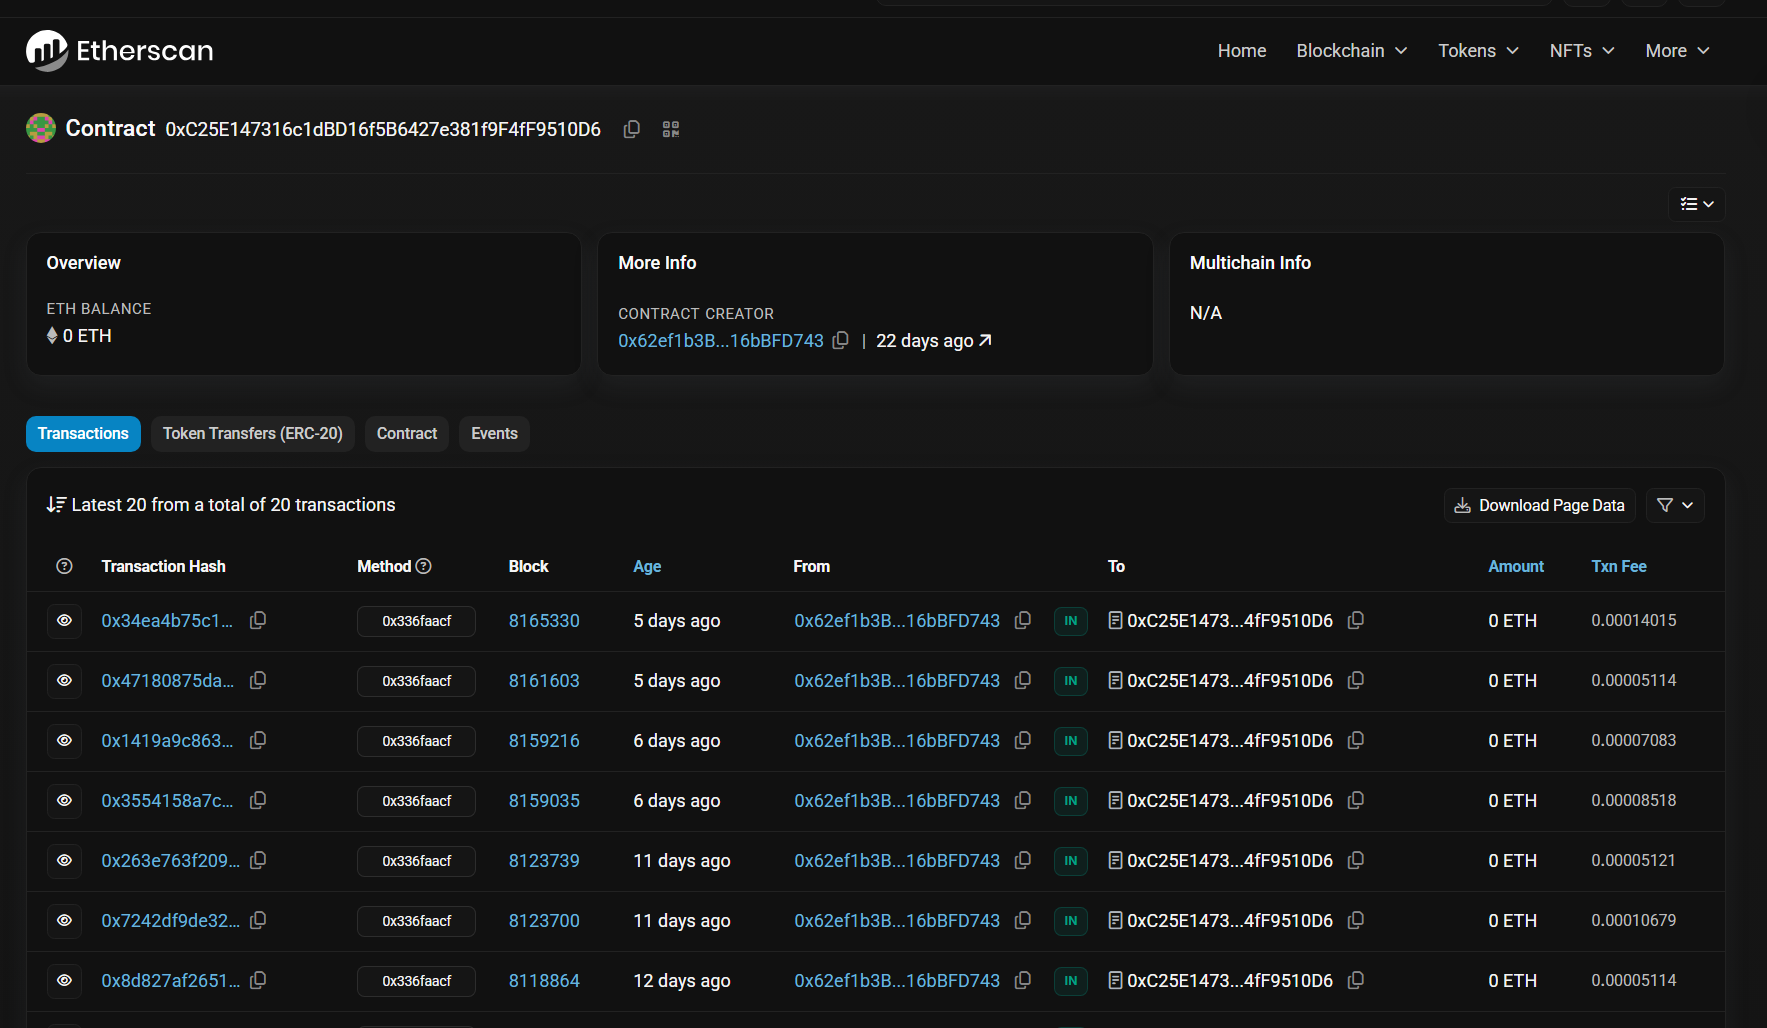
\includegraphics[width=0.8\textwidth]{images/etherscan_screenshot.png}
  \caption{Investment Contract in Etherscan after deployment}
  \label{fig:etherscan-screenshot}
\end{figure}

\subsubsection{Testing}

The testing process used the following tools:

\begin{itemize}
    \item 
\includegraphics[width=0.05\textwidth]{images/icons/remix.png} \textbf{Remix IDE:} For writing, testing, and deploying Ethereum smart contracts
    \item 
\includegraphics[width=0.05\textwidth]{images/icons/hardhat.png} \textbf{Hardhat:} For local blockchain simulation, testing, and deploying contracts
\end{itemize}

The testing approach included:

\begin{itemize}
    \item \textbf{Unit Testing:} Testing core functions individually
    \item \textbf{Integration Testing:} Validating full transaction flows
    \item \textbf{Event Listening:} Capturing and validating event emissions
    \item \textbf{Performance Testing:} Ensuring efficient operation under load \cite{Parizi2018SmartContractProgramming}
\end{itemize}

\newpage
% Placeholder for Smart Contract Deployment & Interaction flowchart
\begin{figure}[htbp]
  \centering
  % PLACEHOLDER: Insert Smart Contract Deployment & Interaction flowchart here
  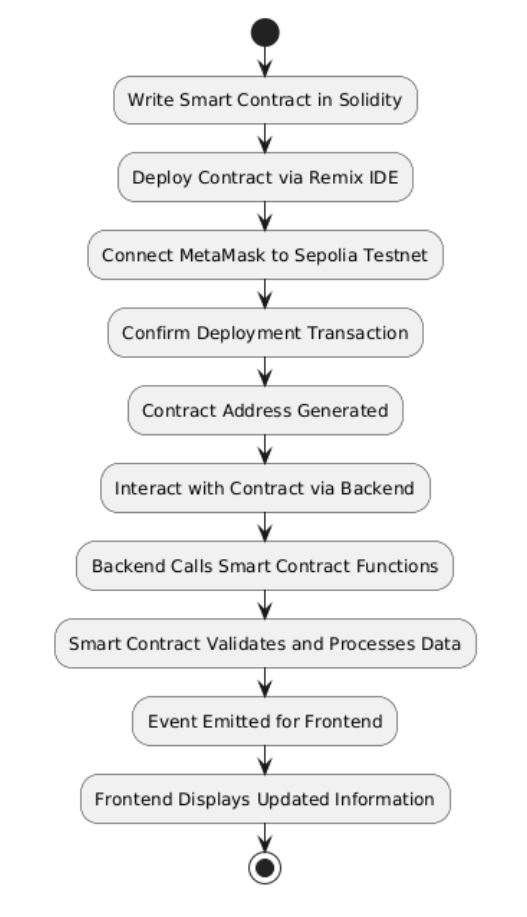
\includegraphics[width=0.8\textwidth]{images/contract_flowchart.png}
  \caption{Flowchart: Smart Contract Deployment \& Interaction}
  \label{fig:contract-flowchart}
\end{figure}

\newpage
% Placeholder for Full Blockchain Deployment Diagram
% \begin{figure}[htbp]
%   \centering
%   % PLACEHOLDER: Insert Full Blockchain Deployment Diagram here
%   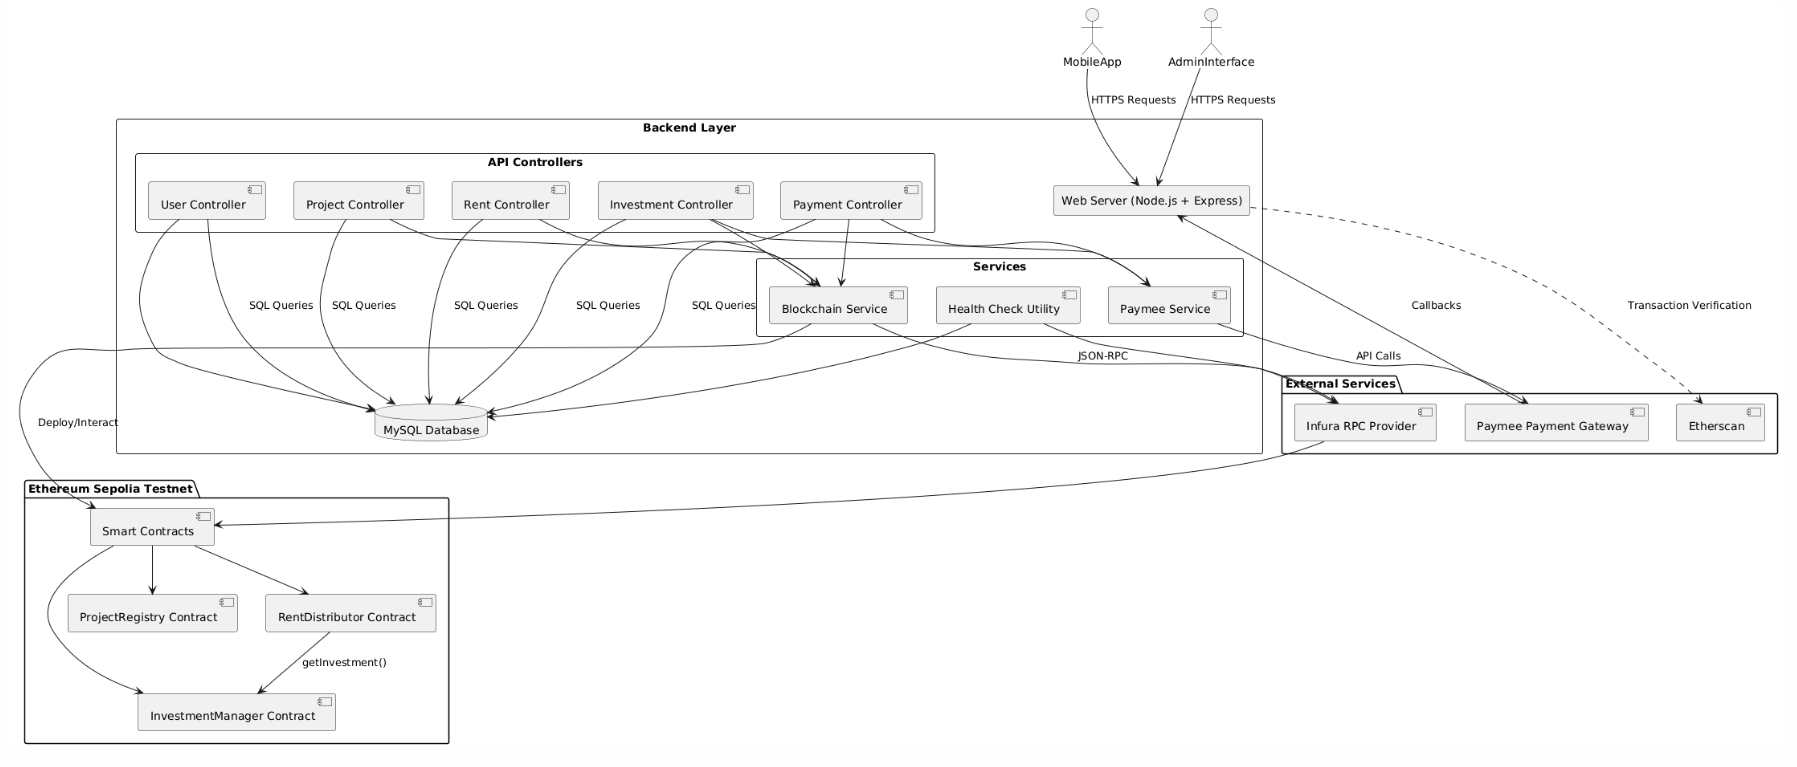
\includegraphics[width=\textwidth]{images/blockchain_deployment_diagram.png}
%   \caption{Full Blockchain Deployment Diagram}
%   \label{fig:blockchain-deployment}
% \end{figure}

\section{Integration Flow}

The integration flow can be summarized as follows \cite{Casino2019BlockchainApplications}:

\subsection{Investment Flow}

\begin{itemize}
    \item The frontend initiates a payment session via Paymee's API
    \item Paymee redirects the user to complete the payment
    \item Upon success, Paymee calls back our backend with the transaction details
    \item After verification, the backend invokes the appropriate smart contract to log the investment on the blockchain
\end{itemize}

% Placeholder for Investment sequence diagram
\begin{figure}[htbp]
  \centering
  % PLACEHOLDER: Insert Investment sequence diagram here
  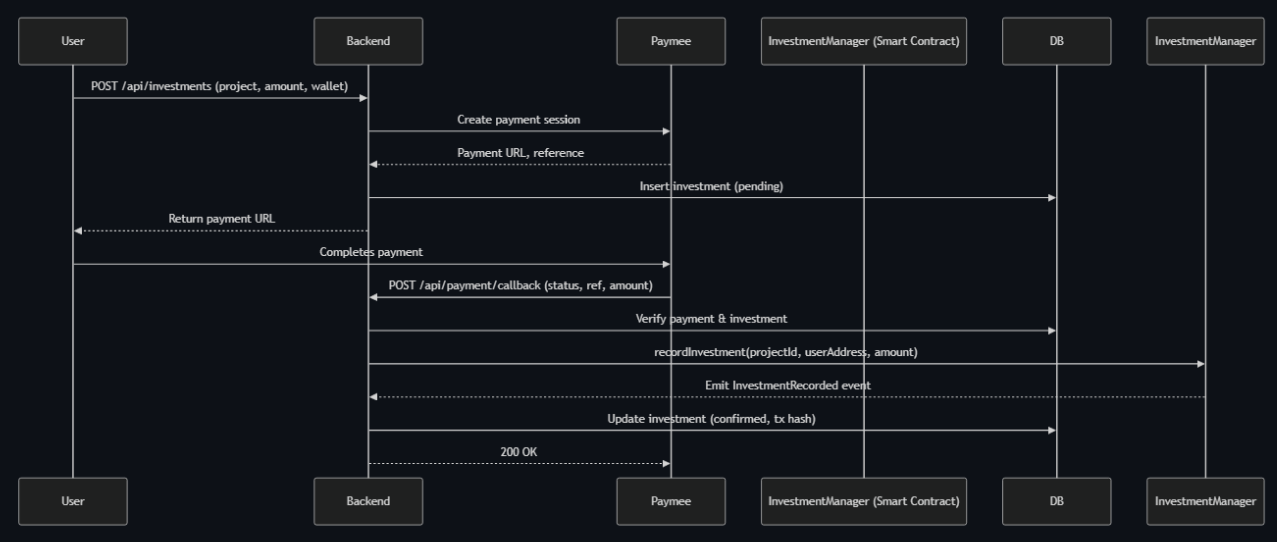
\includegraphics[width=\textwidth]{images/investment_sequence.png}
  \caption{Sequence Diagram of the Investment Process}
  \label{fig:investment-sequence}
\end{figure}

\subsection{Rent Distribution Flow}

\begin{itemize}
    \item The backend initiates the rent distribution process by invoking the smart contract
    \item The smart contract calculates each investor's share based on their investment proportion
    \item For each investor, the smart contract emits an event indicating the calculated share
    \item The backend listens for these events, verifies the data, and triggers the payment through Paymee's API
    \item System records are updated after successful transactions
\end{itemize}

% Placeholder for Rent distribution sequence diagram
\begin{figure}[htbp]
  \centering
  % PLACEHOLDER: Insert Rent distribution sequence diagram here
  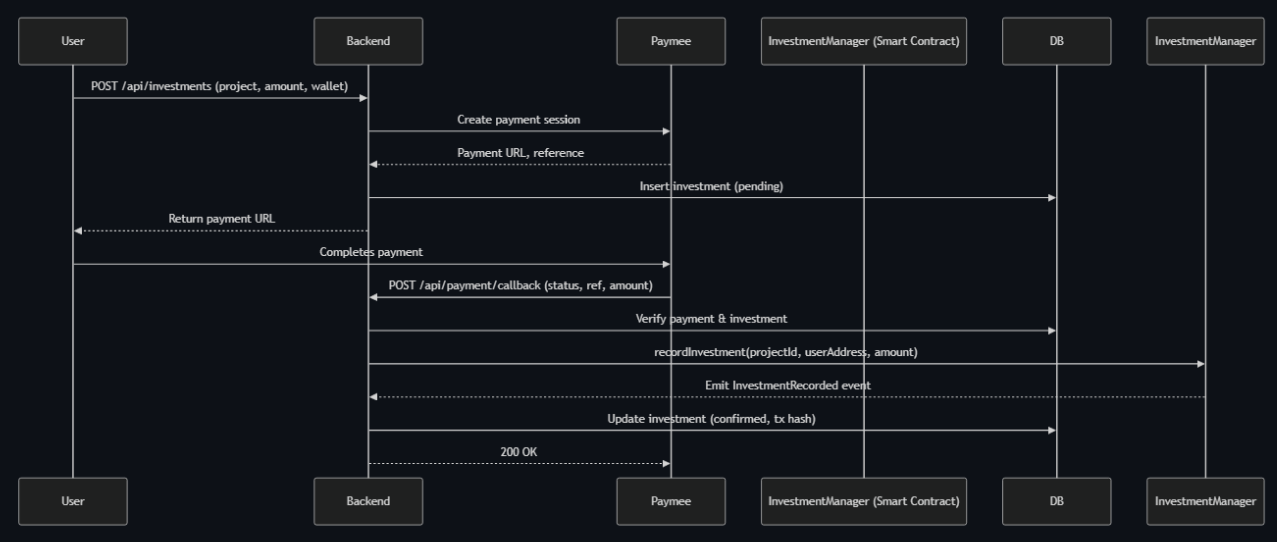
\includegraphics[width=\textwidth]{images/rent_distribution_sequence.png}
  \caption{Sequence Diagram of Rent Distribution}
  \label{fig:rent-distribution-sequence}
\end{figure}

\section{Backoffice Features}

\subsection{Administrative Dashboard}

The backoffice provides administrators with a comprehensive dashboard to manage the platform. Key features include:

\begin{itemize}
    \item Real-time monitoring of blockchain transactions
    \item Project management interface for adding, editing, and removing properties
    \item User management with role-based access control \cite{Botha2021BackofficeBlockchain}
    \item Financial reporting and analytics
    \item Blockchain transaction verification tools
\end{itemize}

% Placeholder for Admin Dashboard screenshot
\begin{figure}[htbp]
  \centering
  % PLACEHOLDER: Insert Admin Dashboard screenshot here
%   \includegraphics[width=0.9\textwidth]{images/admin_dashboard.png}
  \caption{Blockchain Transaction Monitoring in Administrative Dashboard}
  \label{fig:admin-dashboard}
\end{figure}

\subsection{Transaction Management}

Administrators can monitor and manage all types of transactions:

\begin{itemize}
    \item View all investment records with blockchain verification links
    \item Monitor rent distribution status and history
    \item Verify payment processing through the Paymee integration
    \item Generate financial reports and audit trails
\end{itemize}

% Placeholder for Transaction Management Interface
\begin{figure}[htbp]
  \centering
  % PLACEHOLDER: Insert Transaction Management Interface screenshot here
%   \includegraphics[width=0.9\textwidth]{images/transaction_management.png}
  \caption{Transaction Management Interface with Blockchain Verification}
  \label{fig:transaction-management}
\end{figure}

\section*{Conclusion}

The blockchain integration and backoffice features of the Korpor platform provide a robust foundation for secure, transparent, and efficient real estate investment management. By leveraging blockchain technology for critical financial operations while maintaining a user-friendly interface through the backoffice, the platform successfully bridges the gap between traditional finance and decentralized systems \cite{Andoni2019BlockchainOverview}.

The smart contracts deployed on the Ethereum Sepolia Testnet validate core operations such as investment recording and rent distribution, ensuring the accuracy and transparency of financial flows. All interactions are securely handled and recorded on-chain, offering verifiable proof of activity and strengthening participant confidence.

By guaranteeing the integrity of payments and providing clients with clear, tamper-proof records, the blockchain integration significantly enhances user trust and overall satisfaction with the Korpor platform. 